%% Commands for TeXCount
%TC:macro \cite [option:text,text]
%TC:macro \citep [option:text,text]
%TC:macro \citet [option:text,text]
%TC:envir table 0 1
%TC:envir table* 0 1
%TC:envir tabular [ignore] word
%TC:envir displaymath 0 word
%TC:envir math 0 word
%TC:envir comment 0 0
\documentclass[manuscript,screen,review]{acmart}
\AtBeginDocument{%
  \providecommand\BibTeX{{%
    Bib\TeX}}}
\newcommand{\RomanNumeralCaps}[1]
    {\MakeUppercase{\romannumeral #1}}
\usepackage{graphicx}
\usepackage{subfigure}
\usepackage{amsmath}
\usepackage{multirow}
\usepackage{bbding}
\setcopyright{acmlicensed}
\settopmatter{printacmref=true}
\renewcommand\footnotetextcopyrightpermission[1]{}
\acmConference[]{}{}{}
\acmBooktitle{}
\acmPrice{}
\acmDOI{}
\acmISBN{}
\pagestyle{plain}
\acmSubmissionID{2565}



\begin{document}
\title{Improving Recognition of Overlapping Human Speech on Single-Microphone Social Robots with Streaming Two-Mask CMGAN Post-Filtering}

\author{Anonymous for Review}

\begin{abstract}
Recognizing user speech during overlap is important for barge-in handling in human--robot interaction~(HRI). On a single-microphone social robot, this problem becomes difficult when human speech overlaps with the robot's own playback and robot ego-speech filtering~(RESF) is required. Although RESF reduces self-speech interference, subtraction-based filtering can oversuppress the fundamental-frequency range~(FFR) of human speech, which distorts the voiced structure and degrades downstream automatic speech recognition~(ASR).

We address this bottleneck with a streaming Two-Mask CMGAN post-filter applied after RESF. The method combines an additive compensation term to recover oversuppressed structure with a denoising mask to suppress residual interference. To support streaming-compatible operation, we pair the model with sliding-window incremental inference that processes short current blocks while retaining look-back context from previous audio.

We evaluate the method through component-level technical experiments on synthetic overlap mixtures and on lab-recorded Pepper overlap data. On the real Pepper recordings, the proposed pipeline reduces the word error rate from 24.56\% to 10.39\% with \textit{Whisper-large-V3} as the downstream recognizer. Under the profiled server setup, the post-filter runs with a processing factor of 0.015 relative to audio duration on an NVIDIA H100 GPU.

These results support the proposed method as a technical component for overlap-robust speech understanding in single-microphone HRI systems.
\end{abstract}

\begin{CCSXML}
<ccs2012>
   <concept>
       <concept_id>10003120.10003121</concept_id>
       <concept_desc>Human-centered computing~Human computer interaction (HCI)</concept_desc>
       <concept_significance>300</concept_significance>
       </concept>
   <concept>
       <concept_id>10003120.10003123.10010860.10010859</concept_id>
       <concept_desc>Human-centered computing~User centered design</concept_desc>
       <concept_significance>500</concept_significance>
       </concept>
 </ccs2012>
\end{CCSXML}

\ccsdesc[300]{Human-centered computing~Human computer interaction (HCI)}
\ccsdesc[500]{Human-centered computing~User centered design}

\keywords{Human-Robot Interaction, Overlapping Speech Recognition, Robot Ego-Speech Filtering, Speech Enhancement, Streaming Inference}
\maketitle
\fancyhf{}
\renewcommand{\headrulewidth}{0pt}
\fancyfoot[C]{\thepage}
\pagestyle{fancy}

\section{Introduction}
\label{section:1}


Handling overlap is important in HRI because users often attempt to speak while the robot is still talking~\cite{gervits2018pardon,skantze2021turn}. In practice, many robots avoid this situation by disabling the microphone during robot speech, because recognizing overlapping user speech from a single embedded microphone remains unreliable~\cite{Li_2024}. This leaves barge-in handling dependent on conservative turn management rather than on direct access to the linguistic content of the overlap.

This paper addresses a specific front-end bottleneck within that broader HRI problem: recovering recognizable overlapping human speech after robot ego-speech filtering~(RESF) on a single-microphone social robot~\cite{li2024near}. RESF can reduce playback leakage, but subtraction-based filtering can also oversuppress the user's speech in the fundamental-frequency range~(FFR) when robot playback is dominant~\cite{li2024near}. The resulting loss of voiced structure can substantially degrade downstream ASR, even when some higher-frequency information remains available~\cite{braun2022effect}. Figure~\ref{fig:1} illustrates a representative RESF failure case of this kind.
\begin{figure}[htb]
    \centering
    \subfigure[Spectrogram on a linear scale. 
    ]{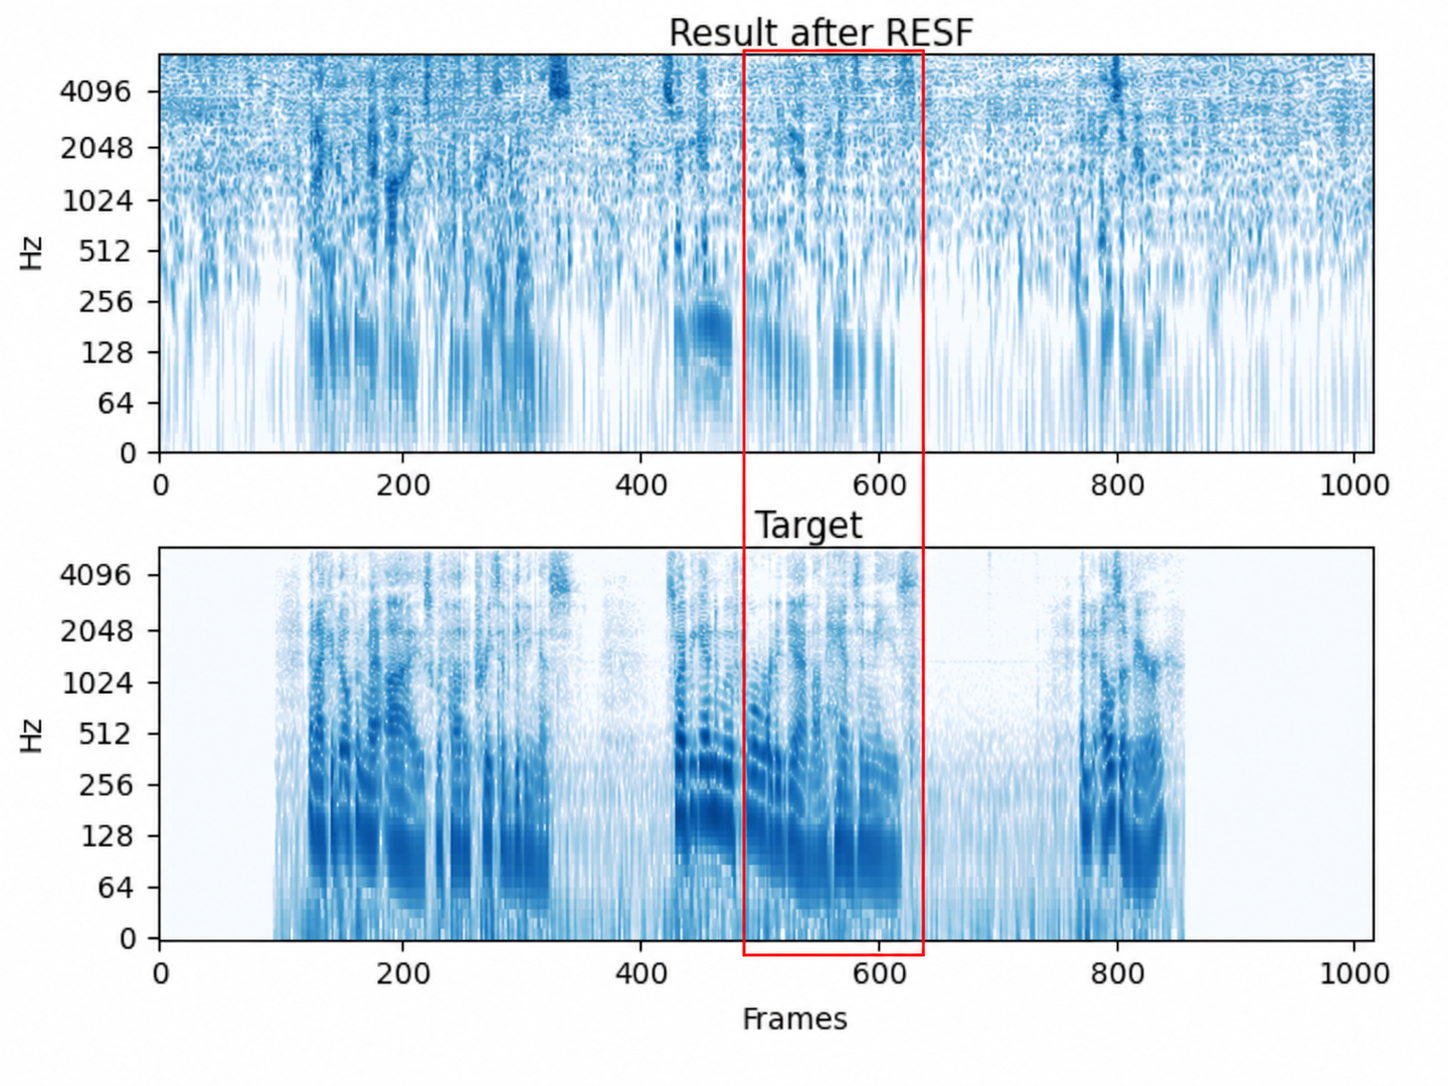
\includegraphics[width=0.45\textwidth]{figs/Comparison_linear.png}}
    \subfigure[Spectrogram on a logarithmic scale. 
    ]{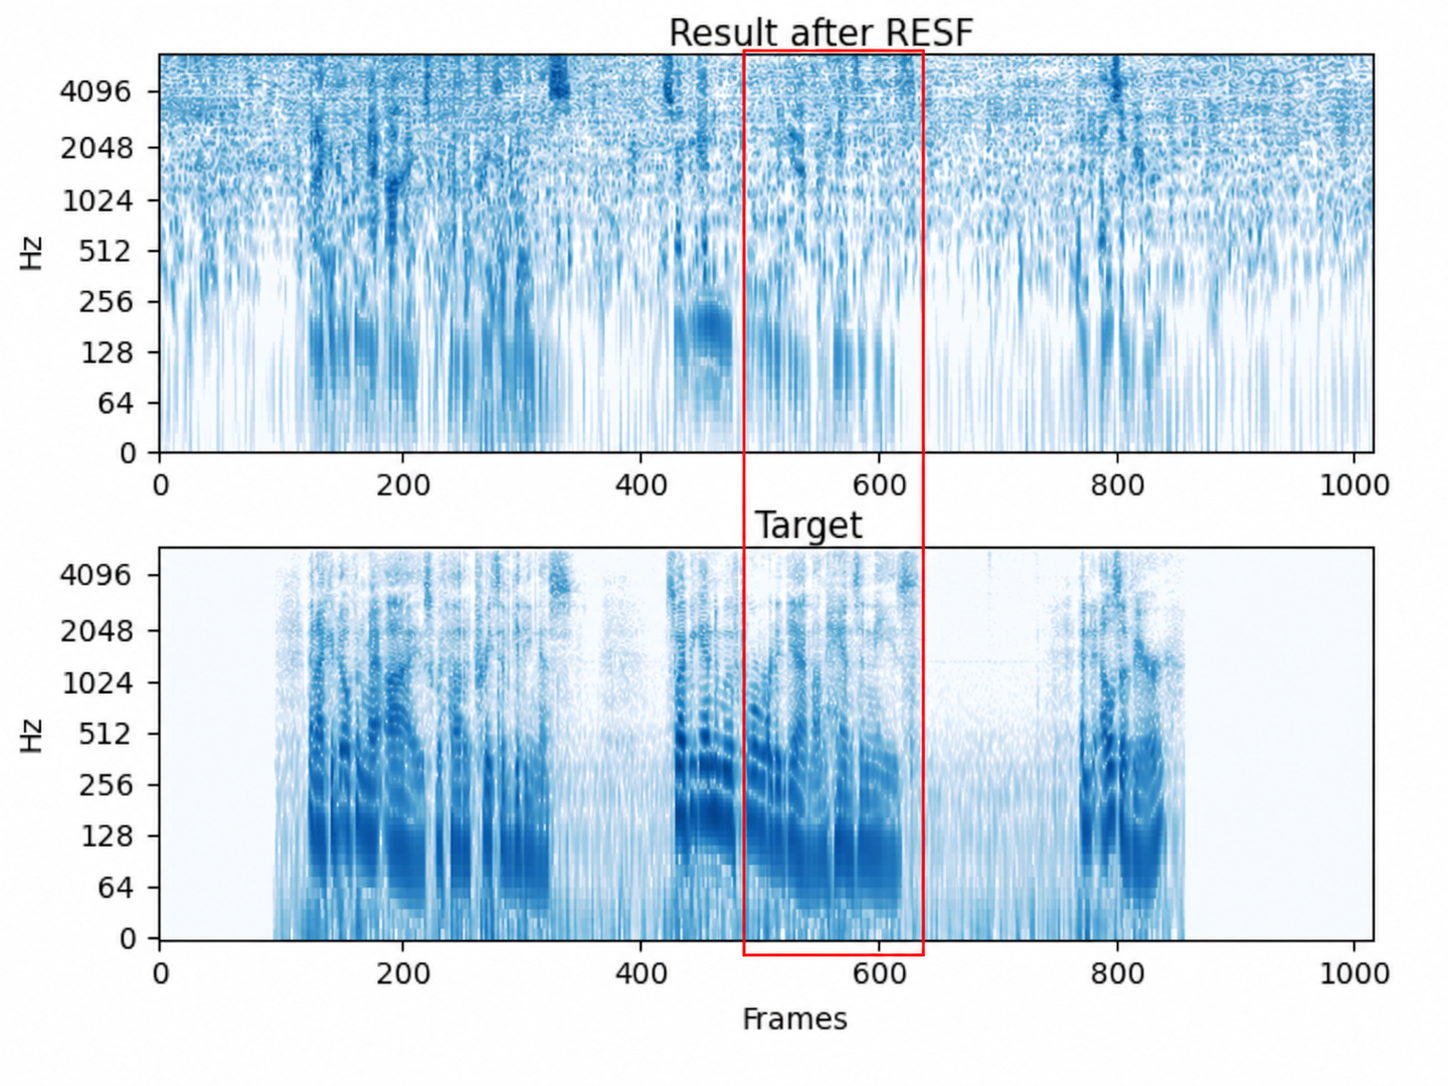
\includegraphics[width=0.45\textwidth]{figs/Comparison_log.png}}
    \caption{Representative RESF failure case. The higher-frequency structure is partly preserved, but oversuppression in the FFR weakens voiced components and leads to a downstream ASR error.}
    \Description{Comparison between a target utterance and the corresponding RESF output. Panel (a) shows the linear-frequency spectrogram and panel (b) shows the log-frequency spectrogram. The highlighted region indicates that the FFR is oversuppressed even though part of the higher-frequency structure remains visible.}
    \label{fig:1}
\end{figure}
The distorted spectrogram should be interpreted as the signal that would be passed from the robot-audition front end to the recognizer after RESF. The energy that remains in regions reflects target speech residuals and the remaining acoustic noise floor after RESF, which becomes especially visible in the logarithmic view. The interaction-relevant failure is instead the weakening of the user’s voiced structure in the low-frequency range while some higher-frequency structure remains visible. In an HRI setting, this matters because the robot may still receive an audio stream during overlap, but the front end has removed part of the speech evidence needed for ASR to recover what the user said.

A central difficulty is that post-RESF audio is not simply noisy speech. As our evaluation later shows, several standard enhancement baselines increase WER relative to the RESF-only signal, indicating that generic suppression can remove or distort recognition-relevant evidence after RESF. This motivates a dedicated post-RESF recovery strategy that can compensate for the oversuppressed voiced structure and denoise the estimate as well.

This bottleneck is not well covered by existing work. HRI studies on interruption and barge-in often focus on detection, overlap classification, or turn-yielding policy~\cite{bekal22_interspeech,selfridge2013continuously,inoue2025yeah}, while speech enhancement research typically targets perceptual quality, generic denoising, or longer-context offline inference~\cite{pascual2017segan,cao2022cmgan,fan2022real}. Less attention has been paid to ASR-oriented recovery of overlapping human speech after RESF-induced oversuppression in a more constrained single-microphone robot setting, where the spatial separation cues used by array-based systems are unavailable. The intended use case is also latency-constrained: during barge-in, the robot should recover usable ASR evidence while the overlap is unfolding, rather than waiting for a complete utterance~\cite{selfridge2013continuously}. So we evaluate the post-enhancement under a streaming-compatible inference pattern that emits short enhanced blocks using only the current block and past acoustic context.

We therefore position this work as a technical contribution to HRI. The primary contribution is a novel algorithmic component for overlap-robust speech recovery on a single-microphone robot, evaluated through component-level technical experiments rather than a systems-level user study. The specific contributions of this work are as follows.


\begin{itemize}
    \item \textbf{HRI-specific technical problem formulation:} we formulate a robot-audition problem focused on recovering the lexical content of overlapping user speech after RESF. It complements the interruption-detection and turn-management work by targeting the front-end speech recovery step needed before downstream ASR on single-microphone social robots \cite{skantze2021turn}.
    \item \textbf{Two-Mask algorithmic contribution:} we propose a post-filter that separates additive compensation for RESF-induced oversuppression from subsequent denoising, with the goal of preserving recognition-relevant voiced structure.
    \item \textbf{Streaming-compatible inference contribution:} we introduce a sliding-window incremental inference scheme that maps Pepper's short audio buffers to a context-aware enhancement window while keeping the evaluation aligned with deployment-motivated streaming use.
    \item \textbf{A component-level evaluation protocol with synthetic and robot-recorded overlap data:} we evaluate the proposed post-RESF speech recovery using paired synthetic RESF-distorted overlap examples under clean/unseen ambient-noise conditions, together with a lab-recorded Pepper overlap set of 90 single-microphone segments from 18 participants. This evaluation design verifies the proposed algorithm's effectiveness, noise robustness, and robot-recorded transfer while keeping the scope distinct from the validation of the live dialog-system.
\end{itemize}

\section{Related Work}

\subsection{HRI interruption and barge-in handling}
Current work on interruption handling in HRI and spoken dialogue systems has mainly focused on detecting overlap and deciding how the robot should react to it~\cite{gervits2018pardon,bekal22_interspeech,selfridge2013continuously,cao2025interruption}. Closely related studies examine backchannels, floor transfer, and timing in human--robot conversation~\cite{skantze2021turn,inoue2025yeah}. This literature establishes why overlap matters for interaction, but it typically treats overlapping speech as a control signal for turn management rather than as speech whose lexical content must still be recovered.

Recovering the lexical content of overlapping user speech is valuable because interruption handling is not only a timing problem, but also an information-preservation problem~\cite{selfridge2013continuously}. A robot that merely detects an interruption may know when to yield the floor but still lacks the linguistic content needed to respond appropriately~\cite{gervits2018pardon}. By contrast, recovering the user's speech during overlap can help the system preserve dialogue context, reduce repair turns caused by missed utterances, and support smoother continuation after overlap detection~\cite{skantze2021turn}. 
% The present paper targets this front-end recovery step and evaluates its downstream effect on complete dialogue behavior remains future work.

\subsection{Robot ego-speech filtering and robot audition}
Robot audition introduces front-end constraints that are closely tied to the interaction setting, including dynamic acoustic scenes, platform-specific acoustics, and limited on-board sensing~\cite{nakadai2012robot}. During robot speech, these constraints become more severe because the microphone signal may also contain strong playback leakage from robot's own speech and other robot-generated noise~\cite{li2024near}. These conditions differ from generic speech enhancement because the front end must support recognition of user speech while the robot itself is an active acoustic source.

A substantial line of robot-audition research has addressed overlapping speech, ego-noise, and environmental interference with microphone arrays or other multichannel processing~\cite{10096344}. Such systems typically combine sound source localization, source separation, post-filtering, and ASR, using spatial information to estimate source directions and separate concurrent acoustic sources~\cite{nakadai2012robot}. More recent work on Pepper has shown that single-channel RESF can expose overlapping user speech from the robot's embedded microphone~\cite{Li_2024,li2024near}. However, after single-channel RESF, the available signal is not an array mixture from which competing sources can still be spatially separated. It is a post-RESF signal in which the recognition-relevant voiced structure may already have been oversuppressed. The resulting problem is therefore not only to suppress interference, but also to recover lexical evidence that has been weakened by the robot-audition front end itself. The present work addresses this gap with a Two-Mask post-filter that separates compensation for RESF-induced oversuppression from subsequent denoising before downstream ASR.
\subsection{ASR-oriented and streaming speech enhancement}
Modern speech enhancement methods such as DCCRN, FullSubNet, SEGAN, MetricGAN, and CMGAN have demonstrated strong results on generic noise suppression and perceptual quality benchmarks~\cite{hu2020dccrn,hao2021fullsubnet,pascual2017segan,fu2019metricgan,cao2022cmgan}. However, improvements in perceptual metrics do not necessarily translate into improved ASR, and enhancement artifacts can even harm recognition~\cite{Donahue2018,iwamoto2022bad,braun2022effect,ristea2024icassp}. In addition, many high-performing attention-based systems rely on relatively long input segments, which complicates deployment in low-latency settings~\cite{fan2022real,drgas2023survey}. Existing HRI work often addresses interruption detection or turn management, while speech enhancement work typically targets generic noise suppression or perceptual quality. The intersection remains underexplored: ASR-oriented recovery of overlapping human speech after RESF on single-microphone robots.

\section{Methods}
\label{Method:SS}
This section describes the RESF front end, the proposed Two-Mask CMGAN-based post-filter, and the streaming-compatible incremental inference procedure used throughout the evaluation.

\subsection{Robot Ego-Speech Filtering}
For single-channel robot audition during overlap, the microphone signal $y(t)$ can be written as:
\begin{equation}
    y(t) = s(t)* h(t) + n(t)
\label{eq:1}
\end{equation}
where $s(t)$ denotes the human target speech, $h(t)$ is the transfer path from the human speaker to the microphone, and $n(t)$ collects competing robot playback and residual acoustic interference at time index $t$.

RESF applies spectral subtraction using a playback reference in order to suppress the robot's own speech. For exposition, we describe this stage in a nonnegative time--frequency magnitude representation:
\begin{equation}
    \hat{S}(tf) = Y(tf) -\hat{N}(tf)
\label{eq:2}
\end{equation}
where $Y(tf)$ denotes the RESF input magnitude at time frame $t$ and frequency bin $f$, $\hat{N}(tf)$ the estimated robot ego-speech magnitude, and $\hat{S}(tf)$ the RESF output magnitude. As reported in ~\cite{li2024near}, RESF often preserves useful higher-frequency structure while oversuppressing voiced energy in the FFR when robot playback dominates the mixture. The post-filter is therefore defined in the same magnitude domain: it takes the RESF output magnitude as input and predicts a corrected target-speech magnitude for later waveform reconstruction.

\subsection{Two-Mask CMGAN}
Conventional deep learning-based speech enhancement commonly predicts a single multiplicative mask:
\begin{equation}
    \hat{S}(tf) = Y(tf) \cdot IRM
\label{eq:3}
\end{equation}
where $IRM$ is an ideal ratio mask~\cite{wali2022generative}. However, in the present problem, a purely multiplicative mask can only attenuate or preserve what remains after RESF. It does not directly address the case where the low-frequency voiced structure has already been removed by oversuppression.

We therefore propose a Two-Mask variant tailored to RESF-induced oversuppression:
\begin{equation}
    \hat{S}(tf) = (Y(tf)+C(tf)) \cdot M(tf)
\label{eq:7}
\end{equation}
where $C(tf)$ is an additive compensation term and $M(tf)$ is a denoising mask. The model implements a serial compensate-then-denoise strategy: it first forms the compensated magnitude $Y(tf)+C(tf)$ and then predicts $M(tf)$ from that compensated representation.

In this formulation, $C(tf)$ is an additive residual term predicted in the same magnitude domain as $Y(tf)$, so it can restore energy that is no longer present after RESF, whereas $M(tf)$ is a multiplicative mask applied after compensation to suppress residual noise and artifacts in a way that remains compatible with standard mask-based enhancement. The first stage is therefore not generic denoising: it uses higher-frequency harmonic and formant cues to infer structure that is likely to have been removed in the FFR, while the second stage regularizes the compensated estimate before waveform synthesis~\cite{fant1971acoustic,titze1998principles,oxenham2023questions,iskarous2010vowel}.

\begin{figure}[th]
    \centering
    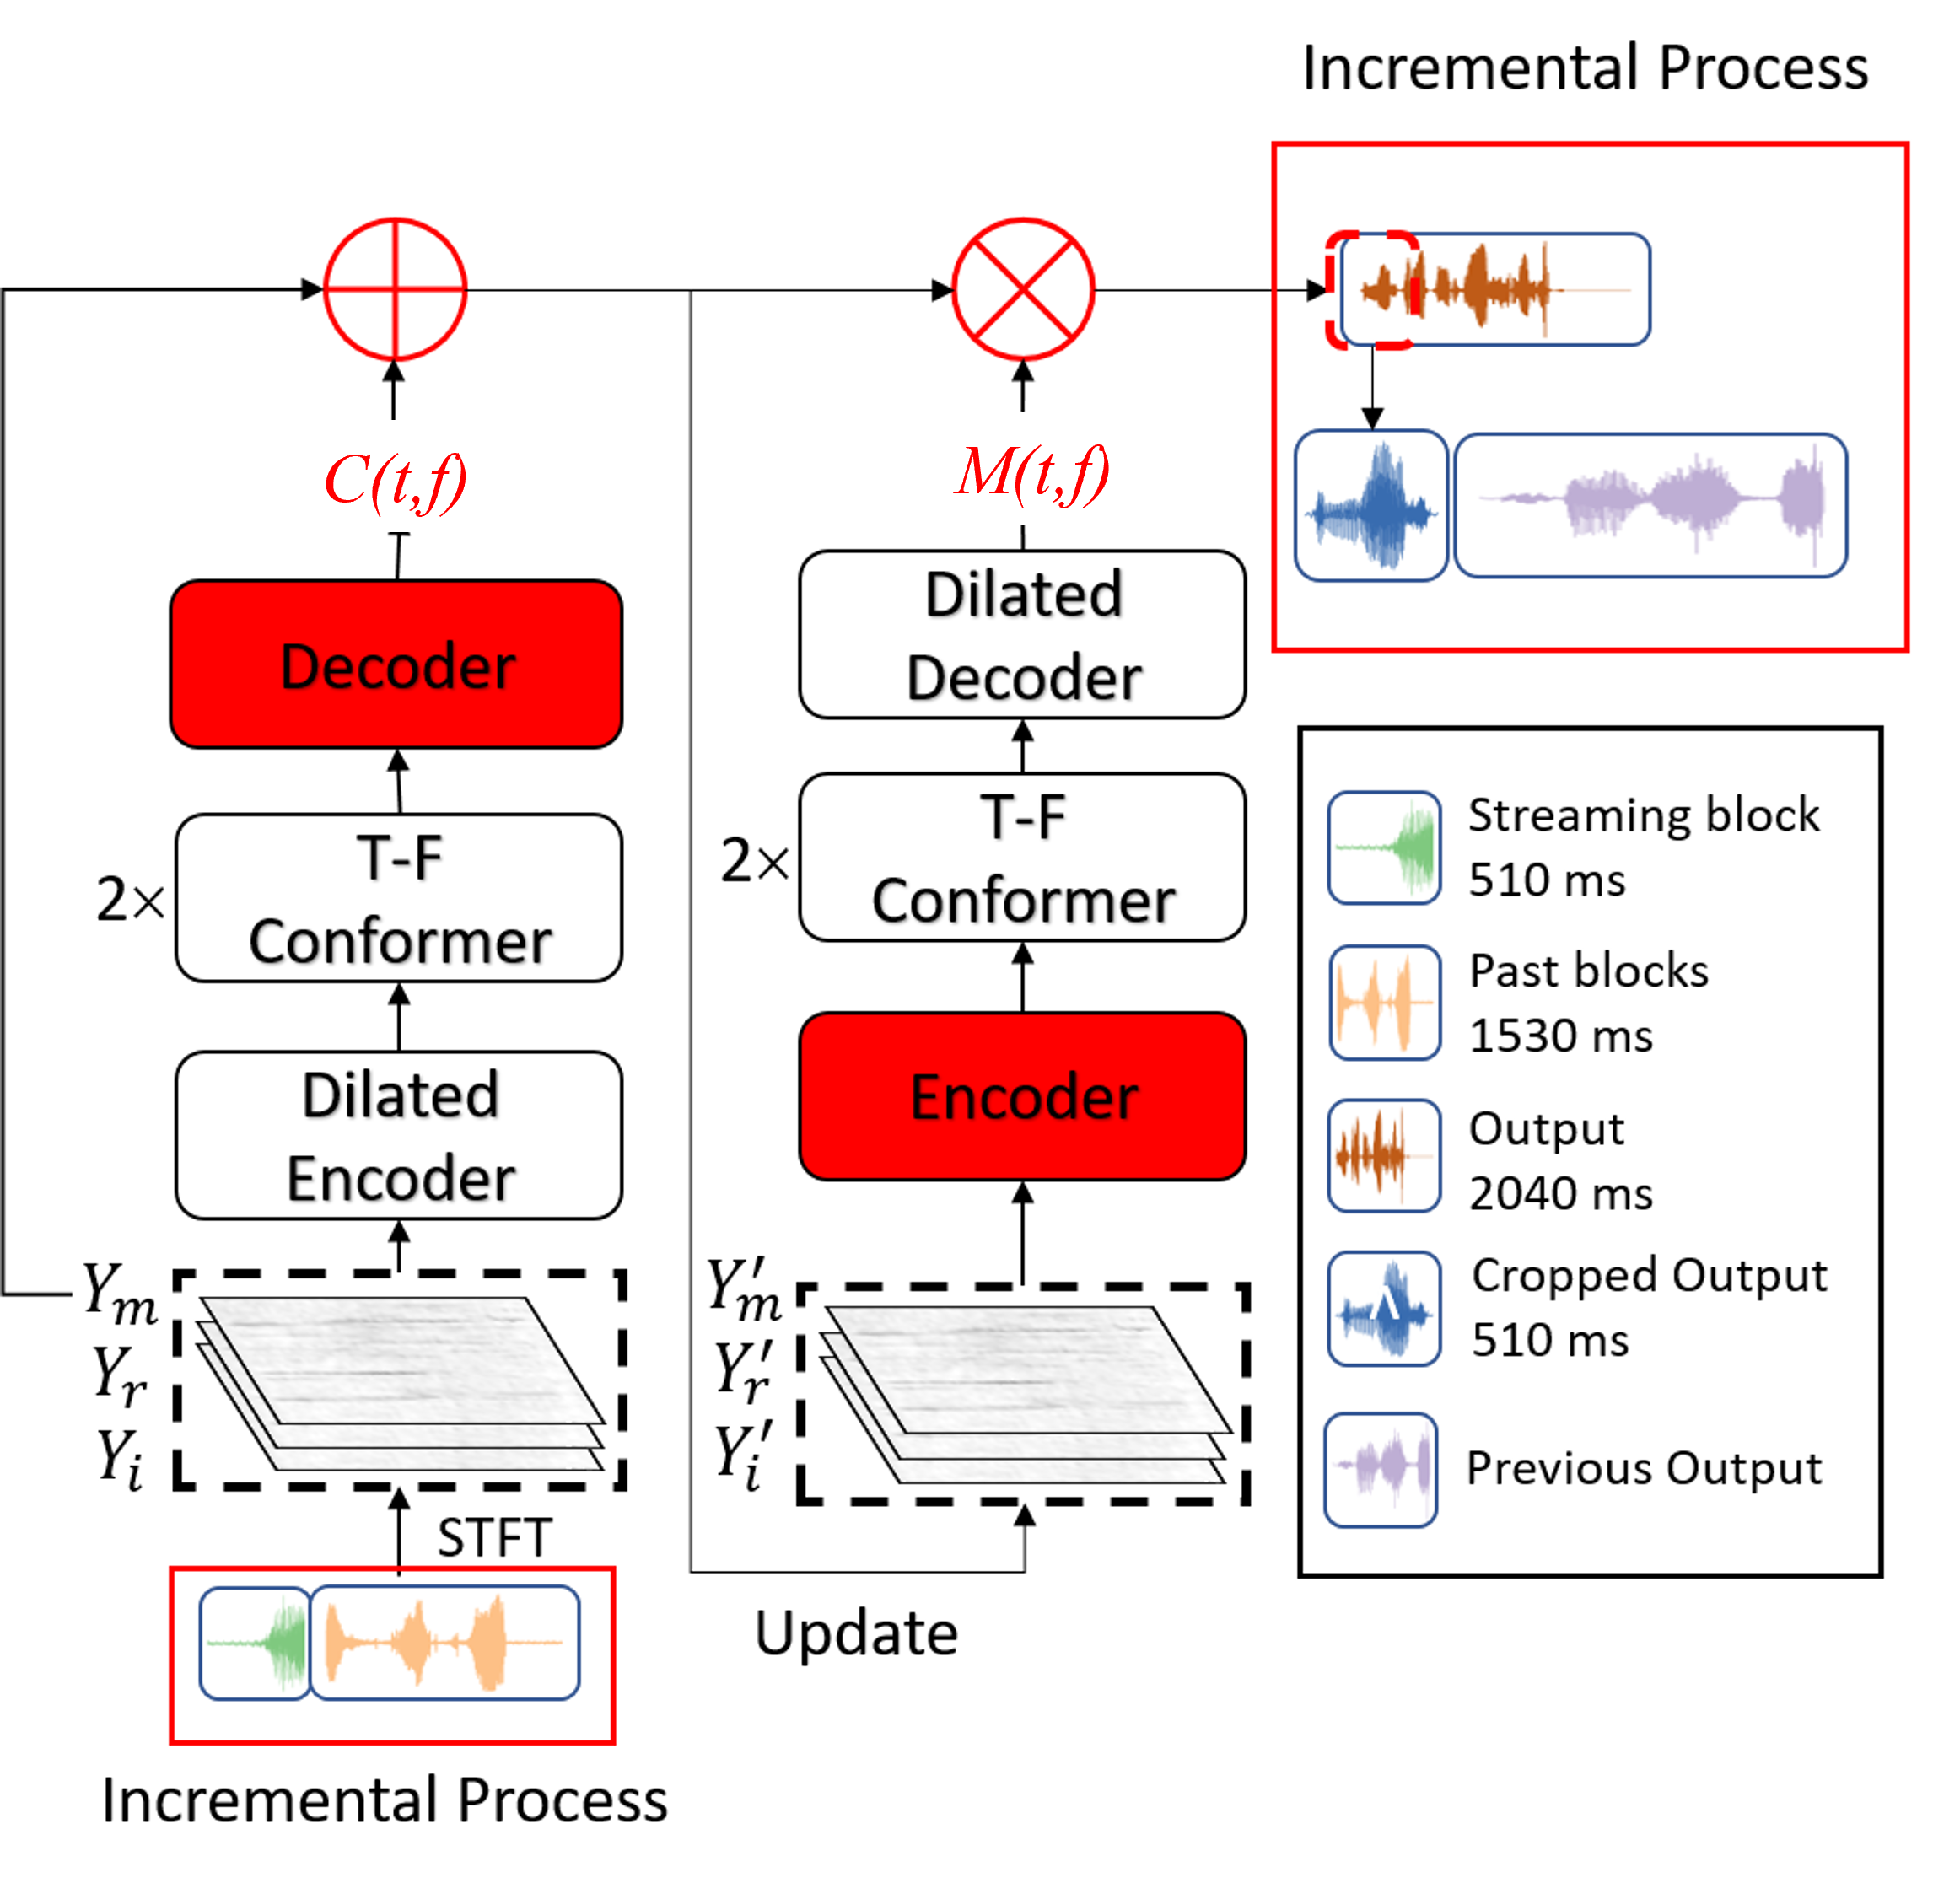
\includegraphics[width=0.7\textwidth]{figs/pipeline_for_se.png}
    \caption{Overview of the proposed Two-Mask post-filter. The shared CMGAN backbone is retained, but the output stage is changed into a sequential two-stage prediction: the generator first estimates an additive compensation term, then predicts a multiplicative denoising mask from the compensated representation, and finally reconstructs the waveform after the second stage.}
    \Description{}
    \label{fig:2}
\end{figure}

Relative to the original CMGAN generator, the shared backbone is retained and only the output-stage behavior is changed so that compensation and denoising have distinct roles, while the adversarial training setup follows the MetricGAN/CMGAN line of work~\cite{Mao_2017_ICCV,cao2022cmgan}. The discriminator operates on 128-bin mel spectrograms instead of the magnitude spectrogram used in the original CMGAN. We use the mel representation because it emphasizes spectral envelope and harmonic organization, which are the cues most affected by RESF-induced oversuppression and most relevant to downstream recognition. The discriminator loss is:
\begin{equation}
\begin{split}
    &\mathcal{L}_{\text{D}} = \mathbb{E}_{X_{\text{mel}},\hat{X}_{\text{mel}}}[\parallel D(X_{\text{mel}}, \hat{X}_{\text{mel}}) - 1 \parallel ^2 ]\\
        &\quad + \mathbb{E}_{X_{\text{mel}}, \hat{X}_{\text{mel}}} [ \parallel D(X_{\text{mel}}, \hat{X}_{\text{mel}}) - Q_{\text{PESQ}} \parallel^2  ] 
\end{split}
\end{equation}
where $D$ is the discriminator, $Q_{\text{PESQ}}$ is the normalized PESQ score in the range $[0,1]$, and $X_{\text{mel}}$ and $\hat{X}_{\text{mel}}$ are the mel spectrograms of the target and enhanced signals. Training is paired: each RESF-distorted input is supervised against its aligned clean human-speech target from the synthetic mixtures described in Section~\ref{Section:Dataset}. This paired setup makes the post-filter specific to RESF-distorted overlap speech rather than to generic noisy speech.

On the implementation side, all audio was processed at 16~kHz. Time-frequency features used a 400-sample analysis window, a 160-sample hop, and a 512-point FFT. The network predicts enhanced magnitudes that are recombined with the corresponding RESF phase for inverse STFT waveform reconstruction. Fixed-length windows are zero-padded where required, including at utterance onset during streaming-compatible inference. Supervision is applied only to the final enhanced output against the aligned clean target. Training followed the CMGAN codebase with AdamW optimization, batch size 4, an initial learning rate of $5\times10^{-4}$, up to 120 epochs, learning-rate decay after epoch 30, and early stopping when the evaluation loss did not improve for five consecutive epochs. We intentionally keep the paper-level implementation description concise; the full training and inference code will be released through our GitHub repository after de-anonymization.


\subsection{Streaming-Compatible Incremental Inference}
\label{Section:Semi-real-time}

% A key deployment challenge is the mismatch between context-hungry enhancement models and the short buffers exposed by robot middleware~\cite{drgas2023survey,fan2022real}. To bridge this gap, we use a sliding-window incremental inference scheme:
As described in Sect.~\ref{section:1}, neural enhancement models often require more acoustic context than the short audio buffers exposed by robot middleware~\cite{drgas2023survey,fan2022real}. This creates a deployment-relevant mismatch for HRI overlap handling, where usable ASR evidence should be recovered while barge-in is unfolding rather than only after a full utterance has been recorded. We address this mismatch with a sliding-window incremental inference scheme based on Pepper's 170~ms NAOqi audio buffers\footnote{\url{http://doc.aldebaran.com/2-5/naoqi/audio/alaudiodevice.html}}.


\begin{enumerate}
    \item \textbf{Current-block formation:} Incoming audio is accumulated until three consecutive 170 ms buffers are available, forming a 510 ms current block.

    \item \textbf{Context-window construction:} The current block is concatenated with the immediately preceding 1530 ms of look-back context, yielding a fixed 2040 ms model input window. At utterance onset, unavailable history is zero-padded so that the input duration remains fixed.

    \item \textbf{Context-aware enhancement:} The Two-Mask CMGAN processes the full 2040 ms window, allowing the model to use recent acoustic context while estimating the enhanced representation for the newest current block.

    \item \textbf{Streaming output and window update:} Only the enhanced samples corresponding to the newest 510 ms current block are retained as the incremental output for later ASR processing. The window then advances by 510 ms: the oldest context is discarded, the previous current block becomes part of the look-back context, and the next incoming block is appended.
\end{enumerate}

From a latency perspective, the relevant emission unit is the 510~ms current block rather than the full 2040~ms model window. The additional 1530~ms is look-back context from already received audio and therefore does not require future look-ahead. After the initial context has been populated, each inference step emits the newest 510~ms block while reusing the previous context. At the level of the enhancement-component, the relevant real-time condition is that each inference step should be completed within this 510~ms emission interval. If this condition holds, the enhancement module processes incoming blocks at least as fast as they arrive and should not, by itself, create a growing buffer backlog. In our profiled server setup, the measured processing factor was 0.015 relative to audio duration, well below the real-time boundary of 1.0. Therefore, we treat the design as low-latency-compatible at the enhancement-component level, while leaving full wall-clock validation across transport, RESF, ASR, and dialogue control to the deployment pathway described later.

 
\section{Experiments}

We evaluate the proposed method as an HRI-relevant technical component. The evaluation targets recognition of overlapping human speech during robot playback rather than full dialogue quality or user experience. The three evaluation sets are organized to assess (i) algorithmic effectiveness on synthetic overlap without added ambient noise, (ii) HRI-specific noise robustness under unseen synthetic background noise, and (iii) robot-relevant transfer evidence on lab-recorded Pepper overlap data.

An overview of the three evaluation sets that were generated as part of the three experiments is presented in Table~\ref{tab:3}.
\begin{table}[ht]
\centering
\caption{Overview of the evaluation sets used for component-level technical evaluation. Set~\RomanNumeralCaps{1} measures algorithmic effectiveness on synthetic overlap without added ambient noise, Set~\RomanNumeralCaps{2} tests noise robustness on unseen synthetic ambient conditions, and Set~\RomanNumeralCaps{3} provides robot-relevant transfer evidence from 90 lab-recorded Pepper overlap segments collected under the tested elicitation protocol.}
\begin{tabular}{lccc}

\hline
 
Evaluation Set & Type           & Ambient Noise               & Number of files \\ \hline
\RomanNumeralCaps{1}              & Synthesis      & \XSolidBrush & 1,000     \\
\RomanNumeralCaps{2}            & Synthesis      & \Checkmark   & 9,033     \\
\RomanNumeralCaps{3}            & Real Recording & \XSolidBrush & 90        \\ \hline
Training Set  & Synthesis           & \XSolidBrush               &9000 \\ \hline
\end{tabular}
\label{tab:3}
\end{table}

\subsection{Experiment 1: Overlapping Speech w/o Ambient Noise}
\label{Section:Dataset}

Experiment 1 evaluates whether the proposed post-filter improves the recognition of overlapping human speech in the clean post-RESF setting, without additional ambient background noise. This experiment uses paired synthetic examples in which the RESF output serves as the distorted post-RESF input, and the aligned clean human speech serves as the target signal.

\subsubsection{Data construction and split}
\label{sec:eval1_data}

As discussed in Section~\ref{section:1}, we are unaware of any public dataset consisting of human speech whose fundamental-frequency range has been oversuppressed by robot ego-speech filtering. We therefore followed the dataset generation scheme of~\cite{Li_2024} and created 10,000 pairs of RESF-distorted overlap examples using the public Robot Voice\footnote{Dataset link is omitted for anonymous review} and LibriSpeech\footnote{\url{https://www.openslr.org/12}} datasets. For each pair, the RESF-processed signal was used as the distorted input, and the clean aligned human speech was used as the target signal.

We randomly assigned 1,000 pairs to \textit{Evaluation Set~\RomanNumeralCaps{1}} and used the remaining 9,000 pairs as the training set. Evaluation Set~\RomanNumeralCaps{1} therefore measures algorithmic effectiveness under controlled overlap conditions without added ambient noise.

\subsubsection{Training and inference set-up}
\label{sec:eval1_setup}

During training, the audio files were randomly cropped to 2040~ms to match the input duration used in CMGAN-style enhancement training~\cite{cao2022cmgan}. At inference time, all methods were evaluated using the same streaming-compatible incremental inference procedure described in Section~\ref{Section:Semi-real-time}, with a 2040~ms context window and a 510~ms output stride. This ensures that the comparison reflects the proposed deployment-motivated inference setting rather than full-utterance offline enhancement.

\subsubsection{Baselines and ablations}
\label{sec:eval1_baselines}

We compared the proposed Two-Mask CMGAN with the classical, neural, and ablation baselines. To compare RESF with a classical front-end signal-processing suppression approach, we included a Wiener filter~\cite{enzner2006frequency} as an acoustic echo cancellation~(AEC) baseline. We also used the ASR output obtained directly from the RESF-processed signal as a RESF-only baseline, allowing us to assess whether each enhancement method improved or degraded downstream recognition relative to RESF alone.

For neural enhancement baselines, we included the pre-trained CMGAN\footnote{\url{https://github.com/ruizhecao96/CMGAN}} and several representative models retrained on our training set: DCCRN~\cite{hu2020dccrn}, Diffusion~\cite{richter2023speech}, SEGAN~\cite{pascual2017segan}, and a retrained single-mask CMGAN. CMGAN is a relevant baseline because it is a conformer-based metric-GAN speech enhancement model designed for time-frequency-domain enhancement~\cite{cao2022cmgan}. To analyze the contribution of the proposed design choices, we further compared the full Two-Mask CMGAN with ablation variants, including a version without incremental processing, a version without the mel-spectrogram discriminator, and an additive-compensation-only variant.

\subsubsection{Evaluation protocol}
\label{sec:eval1_protocol}

The models were evaluated according to how much they improved the downstream recognition of overlapping human speech. Specifically, we applied ASR to each enhanced speech fragment and computed the resulting word error rate~(WER). We adopted \textit{Whisper-large-V3}\footnote{\url{https://openai.com/index/whisper/}} as the ASR backend to transcribe the output of the Wiener filter and RESF baselines, the enhanced output of all neural and ablation models, and the corresponding \textit{Target Speech}.

To reduce dependence on manually prepared transcripts and keep the comparison focused on the effect of enhancement, the ASR transcript obtained from the clean \textit{Target Speech} was used as the reference transcript. We report the mean WER, the corresponding standard deviation and the percentage of files with WER below \textbf{20\%}. We use 20\% WER as a pragmatic success threshold because this roughly corresponds to no more than two word errors in a 10-word utterance. It is also broadly consistent with previous work suggesting that moderate ASR error at this level may still support downstream speech-understanding tasks, whereas higher error rates increasingly require more robust recovery mechanisms~\cite{tejedor2022towards}.

All training, enhancement inference, and ASR evaluation were performed on a server equipped with an NVIDIA H100 GPU. The enhancement models were implemented and evaluated in the same PyTorch-based software environment across all three experiments. 

\subsection{Experiment 2: Overlapping Speech with Ambient Noise}

\subsubsection{Data: Evaluation Set \RomanNumeralCaps{2}}
To assess noise robustness within unseen synthetic ambient conditions that are relevant to HRI, we added fragments from the Microsoft Scalable Noisy Speech Dataset~(MS-SNSD)~\cite{reddy2019scalable}. Specifically, we mixed 61 clean human speech audio files with 17 types of challenging and non-stationary noise from MS-SNSD. These can be categorized into six groups:
\begin{enumerate}
    \item %\textit{Group One:} 
    \textbf{Airport:} AirportAnouncement;
    \item %\textit{Group Two~(
    \textbf{Babble Speech:} 
    Babble, NeighborSpeaking;
    \item %\textit{Group Three~(
    \textbf{Noisy Indoor:} 
    Cafe, Cafeteria, Restaurant, LivingRoom;
    \item %\textit{Group Four~   
    \textbf{Tranquil Indoor:} Copier, Kitchen, Office, Hallway, Typing;
    \item %\textit{Group Five~(
    \textbf{Outdoor:} Park, Square, Station, Traffic;
    \item %\textit{Group Six:} 
    \textbf{Vacuum cleaner:} VacuumCleaner
\end{enumerate}
Given the provided toolkit~\footnote{https://github.com/microsoft/MS-SNSD}, all noisy speech clips were scaled to have nine global SNRs of ${40,35,30,25,20,15,10,5,0}$~dB each. We then created noisy overlapping human--robot speech following the same generation scheme as in Section~\ref{Section:Dataset}. 

% These noisy overlapping speech segments were cut into 2,040~ms blocks with 510~ms hopping distance and fed into the RESF pipeline to obtain the distorted human speech estimation blocks as described in Section~\ref{Section:Semi-real-time}. 

\subsubsection{Experimental set-up}
We compared the proposed Two-Mask CMGAN to the retrained single-mask CMGAN on each noise scenario in Evaluation Set~\RomanNumeralCaps{2}. The inputs were processed with the same 2040~ms window and 510~ms stride described in Section~\ref{Section:Semi-real-time}. All ambient noises in this set are absent from the training set. The ASR procedure was identical to that used for the Evaluation Set~\RomanNumeralCaps{1}, and the average WER was reported for each noise scenario and SNR.
% The performance of the models in improving the interpretation of the detected human interruption speech was evaluated by calculating the WER after applying ASR to the enhanced sound fragment. 


\subsection{Experiment 3: Lab-Recorded Pepper Overlap Evaluation}

\subsubsection{Data: Evaluation Set \RomanNumeralCaps{3}}
\label{subsec:eval3}
% The purpose of this evaluation set was to collect lab-recorded Pepper overlap data and then evaluate the enhancement pipeline offline. We focused on speech segments in which a participant intentionally spoke over the robot, so that the resulting recordings would expose the RESF and post-filter stages to realistic robot self-speech overlap under a controlled elicitation protocol on a single-microphone social robot. Enhancement and ASR were not performed on-device during interaction; the present evaluation is strictly offline and component-level. 
% Evaluation Set~\RomanNumeralCaps{3} should therefore be interpreted as robot-relevant transfer evidence from 90 lab-recorded Pepper overlap segments collected in a controlled, cue-based protocol.

Evaluation Set~\RomanNumeralCaps{3} aims to assess how the proposed post-filter performs on real overlapping speech input recorded during HRI, beyond the controlled synthetic mixtures used in Evaluation Sets~\RomanNumeralCaps{1} and~\RomanNumeralCaps{2}. In particular, this set provides robot-recorded transfer evidence for whether the RESF~$\rightarrow$~post-filter pipeline can improve recognition when a participant speaks over Pepper's own speech through the robot's embedded single-microphone audio channel.

We recorded lab-based Pepper overlap data under a controlled elicitation protocol. Participants intentionally spoke over the robot during Pepper's own speech, producing overlapping recordings that exposed the RESF and post-filter stages to real robot self-speech overlap while keeping the interaction setting experimentally controlled. The recorded overlapping speech was then used for subsequent enhancement and ASR evaluation.


We recruited 18 fluent English speakers from the campus community, 11 women and 7 men aged 26 to 42. We oversampled women because the earlier RESF$\rightarrow$ASR pipeline in~\cite{li2024near} showed worse recognition on female speech than on male speech. All participants provided their informed consent prior to recording.

To elicit overlap, we used a debate scenario in which the participant was instructed to interrupt the robot and continue speaking during robot playback. We prepared 20 topics with paired \textit{Support} and \textit{Against} arguments so that Pepper's spoken segment exceeded 20 seconds at a normal speaking rate.

During the procedure, the human participant sat/stood 0.6-0.8~m in front of the robot Pepper~\cite{weisser2021conversational}. Each participant was asked to interrupt the robot on five different topics, leading to five recordings per participant. At the start of a session, the participant selected five indices from 0 to 19, and the corresponding topics were displayed on Pepper’s tablet. For each chosen topic the participant selected a stance, supporting or against, and Pepper automatically adopted the opposite stance. The participant was given 10 seconds to prepare its arguments with no less than 2 sentences. Pepper then opened its microphone stream and began delivering its argument. To introduce randomness, the tablet displayed a \textit{BARGE IN} cue in a dynamically sampled time per segment, uniformly between 1 second after Pepper started speaking and 50\% of Pepper’s planned utterance duration. After seeing the cue, the participant barged in freely without an imposed lexical or rhetorical pattern. Participants were instructed to finish their arguments regardless of whether Pepper finished its speech. Because Pepper’s arguments exceeded 20 seconds, human entry time ensured an overlap that typically exceeded 10 seconds and, in many cases, covered nearly the remainder of Pepper's speech. 
This procedure resulted in 90 lab-recorded overlapping speech segments, corresponding to five overlap recordings from each of the 18 participants. These 90 segments constitute Evaluation Set~\RomanNumeralCaps{3} and were used for the following enhancement and ASR evaluation.

The audio was captured from Pepper's embedded single microphone using the same acquisition settings as in the synthetic experiments. Recording continued until both speakers had finished and was stored on a local server. The audio stream was controlled by a WebRTC voice activity detector~(VAD)\footnote{\url{https://pypi.org/project/webrtcvad-wheels/}} configured to open on the first speech-active segment and close only after sustained silence. Under our seating distance and loudness conditions, we did not observe premature cut-offs. The experimental scripts and prompt materials are omitted here for anonymous review and can be released in a non-anonymous version.



\subsubsection{Evaluation}
All enhancement and recognition were performed offline on the same server, using the same RESF and Two-Mask CMGAN configurations as in Experiments~1 and~2. The measured post-filter processing factor was 0.015 relative to audio duration. We compared the RESF $\rightarrow$ASR baseline with the RESF $\rightarrow$ Two-Mask CMGAN $\rightarrow $ ASR, the RESF $\rightarrow$ Retrained DCCRN $\rightarrow$ ASR, and the RESF $\rightarrow$ Retrained CMGAN $\rightarrow$ ASR pipelines using the same 2040~ms window and 510~ms stride described in Section~\ref{Section:Semi-real-time}. 

We evaluated the pipelines on the recognized human speech content within each overlap segment. For each segment, we computed WER against a manually prepared reference transcript using the same ASR backend as in the other experiments. We report the mean and standard deviation of WER, the percentage of segments with WER lower than 20\%, and the mean and standard deviation of recognized transcript length in words. 





\section{Results}

\subsection{Evaluation Set~\RomanNumeralCaps{1}}

\begin{table}[ht]
\centering
\caption{Component-level ASR evaluation on \textit{Evaluation Set \RomanNumeralCaps{1}}. All methods are compared with the same downstream ASR and transcript alignment procedure; streaming-compatible incremental inference is enabled unless noted otherwise.}
\begin{tabular}{llccc}
\hline
\multirow{2}{*}{Model} & \multirow{2}{*}{} & \multicolumn{3}{c}{WER~/\%} \\
 &  & Mean & STD & $\leq 20\%$  \\ \hline
Wiener Filter & \multicolumn{1}{c}{-} & 36.56 & 70.24 & 51.12  \\
RESF & \multicolumn{1}{c}{-} & 14.43 & 7.69 & 75.55 \\
DCCRN & \multicolumn{1}{c}{Retrained} & 85.10 & 30.39 & 2.08 \\
Diffusion & \multicolumn{1}{c}{Retrained} & 33.16& 27.75 & 40.86  \\
SEGAN & Retrained & 31.41 & 26.80 & 41.00 \\
 & w/o IP & 40.21 & 25.29 & 24.20 \\
 
CMGAN & Original & 30.34 & 28.49 & 44.86 \\
 & Retrained & 10.29 & 6.06 & 84.99 \\
 & w/o IP & 11.35 & 10.08 &  81.99   \\
& Add & 95.96 & 14.47 &  0.11 \\
Two-Mask  & Proposed & \textbf{7.44} & \textbf{3.92} & \textbf{91.40} \\
 CMGAN& w/o IP & 12.30 & 14.14 & 78.92 \\
 & w/o mel & 9.56 & 5.26 & 86.00 \\ \hline
\end{tabular}
\label{tab:1}
\end{table}
Table~\ref{tab:1} presents the results of Experiment~\ref{Section:Dataset} on Evaluation Set~\RomanNumeralCaps{1}, which tests post-RESF speech recovery under synthetic overlap conditions without added ambient noise. Three main patterns can be seen from the table. 

The first and most important pattern is negative: most generic enhancement baselines do not improve the RESF signal and instead increase WER. Compared with the RESF-only baseline, the Wiener filter, retrained DCCRN, retrained Diffusion model, retrained SEGAN, and original CMGAN all perform worse. This indicates that post-RESF recovery is not equivalent to generic noise suppression. The input has already been shaped by RESF, and additional enhancement can remove or distort recognition-relevant evidence unless the model is adapted to the RESF distortion pattern. By contrast, retraining a single-mask CMGAN on RESF-distorted speech improves mean WER from 14.43\% to 10.29\%, and the proposed Two-Mask CMGAN improves further to 7.44\%. This supports the need for both RESF-specific adaptation and explicit compensation.

Second, additive compensation and denoising play different roles. The additive-only variant fails badly with a mean WER of 95.96\%, which supports the need for denoising after compensation. At the same time, the proposed Two-Mask CMGAN model improves over the retrained single-mask CMGAN from 10.29\% to 7.44\% mean WER and raises the WER $\leq 20\%$ rate from 84.99\% to 91.40\%, which supports the need for an explicit compensation stage when RESF has removed voiced structure.

Third, the streaming-compatible design choices contribute independently. Removing the mel-spectrogram discriminator worsens the mean WER from 7.44\% to 9.56\%, and removing incremental inference worsens it to 12.30\%. Taken together, Set~\RomanNumeralCaps{1} supports the full Two-Mask configuration as the strongest component-level design among the tested alternatives.
\begin{figure}[ht]
    \centering
    \subfigure[Proposed Two-Mask CMGAN]{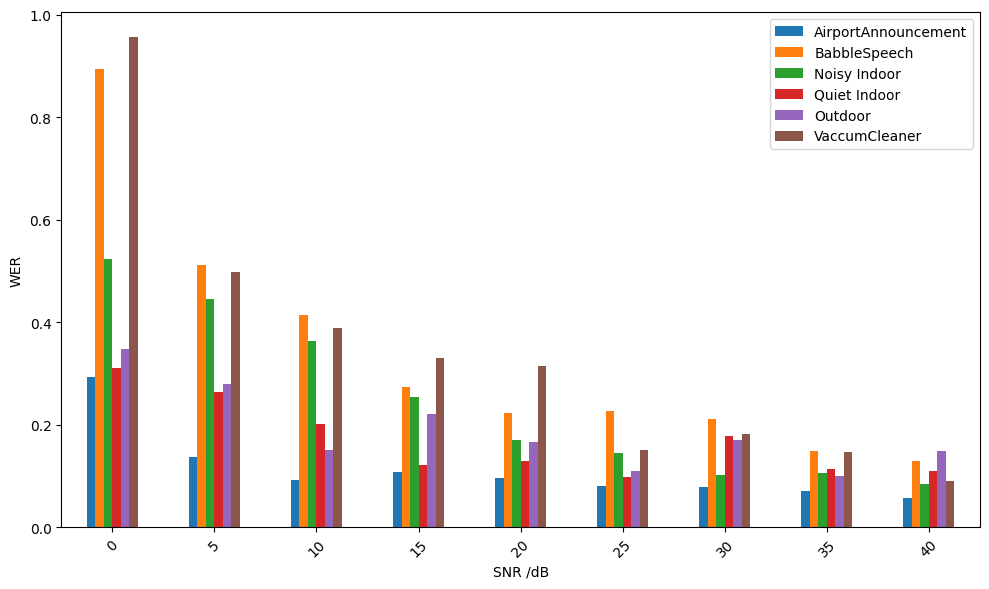
\includegraphics[width=0.43\textwidth]{figs/set2.png}}
    \subfigure[Retrained CMGAN]{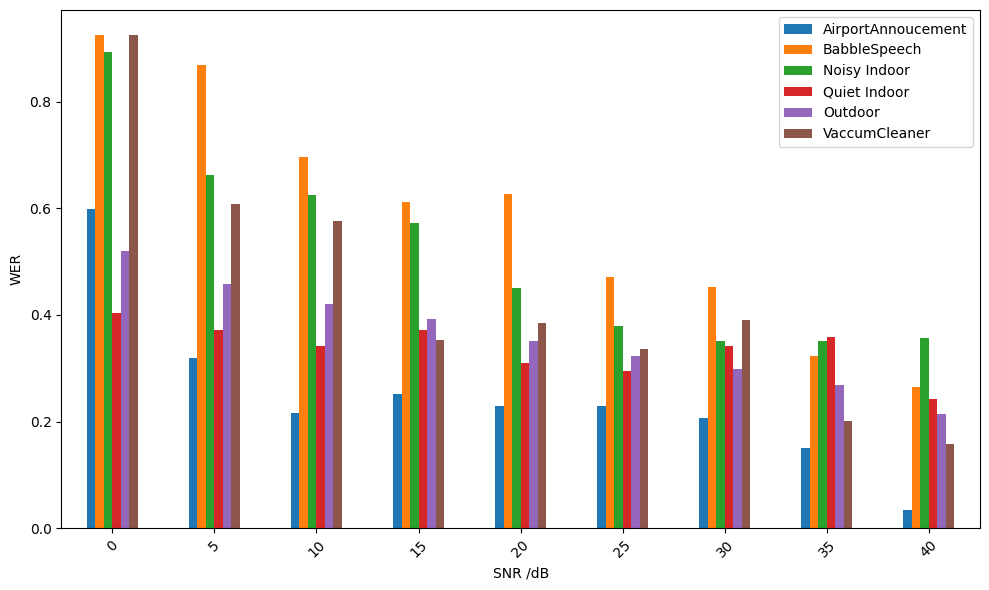
\includegraphics[width=0.43\textwidth]{figs/set3.png}}
    \caption{Average WER on \textit{Evaluation Set \RomanNumeralCaps{2}} across the six HRI-relevant unseen noise families and nine global SNR conditions from 0 to 40~dB. Both panels use the same RESF front end and ASR protocol, enabling a direct component-level comparison between the proposed Two-Mask post-filter and the retrained single-mask CMGAN.}
    \Description{}
    \label{fig:3}
\end{figure}

\subsection{Evaluation Set~\RomanNumeralCaps{2}}

\begin{table}[ht]
\centering
\small
\caption{Summary statistics for \textit{Evaluation Set \RomanNumeralCaps{2}} aggregated by the six HRI-relevant noise families listed in the data description above and by representative SNR levels. Lower WER is better. $\Delta$ denotes the absolute WER reduction of the proposed model relative to the retrained single-mask CMGAN.}
\begin{tabular}{lccc}
\hline
Condition & Retrained & Proposed & $\Delta$ \\
 & CMGAN & Two-Mask &  \\ \hline
\multicolumn{4}{l}{\textit{Noise family averages}} \\
Airport & 40.63 & 25.36 & 15.27 \\
Babble Speech & 54.69 & 37.86 & 16.83 \\
Noisy Indoor & 48.23 & 35.76 & 12.47 \\
Tranquil Indoor & 42.91 & 32.16 & 10.75 \\
Outdoor & 33.39 & 28.49 & 4.90 \\
Vacuum cleaner & 56.53 & 28.63 & 27.90 \\
Macro average & 43.52 & 33.92 & 9.60 \\ \hline
\multicolumn{4}{l}{\textit{Representative SNR averages}} \\
0 dB & 73.63 & 56.93 & 16.70 \\
10 dB & 47.51 & 36.86 & 10.64 \\
20 dB & 33.90 & 27.54 & 6.35 \\
30 dB & 31.67 & 23.04 & 8.63 \\
40 dB & 26.28 & 22.23 & 4.05 \\ \hline
\end{tabular}
\label{tab:set2_summary}
\end{table}

Figure~\ref{fig:3} and Table~\ref{tab:set2_summary} report the noise robustness results on Evaluation Set~\RomanNumeralCaps{2} under unseen synthetic ambient conditions. When averaged within the six HRI-relevant noise families, the proposed Two-Mask model improves over the retrained single-mask CMGAN in every family and lowers the macro-average WER from 43.52\% to 33.92\%, an absolute reduction of 9.60 points. The largest family-level gains appear in Vacuum cleaner (27.90 points), Babble Speech (16.83 points), and Airport (15.27 points), while consistent improvements are also observed in Noisy Indoor (12.47 points), Tranquil Indoor (10.75 points), and Outdoor (4.90 points).

Across SNR conditions, the proposed model remains better at every tested level from 0 to 40~dB. The absolute WER reduction ranges from 4.05 points at 40~dB to 16.70 points at 0~dB, with improvements between 5 and 11 points across the intermediate SNRs. This pattern suggests that the compensate-then-denoise formulation is not tied to a single operating point: it helps both when the RESF output is heavily degraded and when the ambient noise is more moderate.

The most difficult conditions remain Babble Speech and Noisy Indoor, where average WER is still 37.86\% and 35.76\%, respectively. These scenes combine speech-like interference or highly non-stationary indoor activity with the RESF distortion, which makes it harder to recover missing voiced structure without introducing artifacts. This is precisely the type of overlap setting that matters in HRI, because shared public spaces often contain competing talkers and cluttered indoor acoustics. Set~\RomanNumeralCaps{2} therefore extends the evidence from clean synthetic mixtures to noise robustness within the tested synthetic conditions while also clarifying where the operating envelope remains challenging.

\subsection{Evaluation Set~\RomanNumeralCaps{3}}
\begin{table}[ht]
    \centering
    \caption{Offline server-side component-level ASR evaluation on 90 lab-recorded Pepper overlap segments (\textit{Evaluation Set \RomanNumeralCaps{3}}). Mean WER, its standard deviation, the proportion of segments with WER $\leq 20\%$, and recognized transcript length are reported under identical RESF front-end and ASR settings.}
    \begin{tabular}{cccccc}
    \hline
        & \multicolumn{3}{c}{WER~/\%} & \multicolumn{2}{c}{Num\_words}\\
        & Mean~$\downarrow$       & STD~$\downarrow$   & $\leq 20$~$\uparrow$     & Mean          & STD            \\ \hline
RESF + ASR  & 24.56    & 18.39  & 45.88 & 46.27           & 28.13         \\
Two-Mask CMGAN & 10.39    & 8.60   & 83.53 & 47.45           & 28.07         \\ 
Retrained CMGAN & 56.32    & 34.27 & 5.88 &     45.16         &     32.72            \\
Retrained DCCRN &35.22   & 42.76   & 35.29  & 46.28             &  29.95               \\
Ground Truth & - &- &- & 49.79 & 29.62 \\
\hline
    \end{tabular}
    \label{tab:2}
\end{table}

Table~\ref{tab:2} reports the lab-recorded Pepper overlap evaluation on 90 segments collected under the controlled elicitation protocol. The proposed RESF$\rightarrow$Two-Mask CMGAN$\rightarrow$ASR pipeline reduces mean WER to 10.39\%, a 57.7\% relative reduction from the RESF-only baseline. It also lowers the WER standard deviation to 8.60\% and increases the proportion of segments with WER $\leq 20\%$ from 45.88\% to 83.53\%. A paired bootstrap analysis based on segment-level WER differences estimates a mean absolute reduction of 14.16 points with a 95\% confidence interval of [10.23, 18.51]. A two-sided paired sign test further shows that 67 segments improved and 7 worsened, indicating that the gain is broad and not driven by a small number of favorable cases. Because recognized transcript length remains stable across systems, these gains are unlikely to be explained by trivial truncation.

This real-data result is not a case where any enhancement helps equally. The RESF-only baseline yields a mean WER of 24.56\% with a standard deviation of 18.39\%, which indicates that recognizing overlapping human speech during robot playback remains difficult even after robot ego-speech filtering. Adding enhancement on top of RESF does not by itself solve this problem: retrained DCCRN reaches 35.22\% mean WER, and the retrained single-mask CMGAN reaches 56.32\%, suggesting that these models can destabilize badly on real RESF-distorted Pepper recordings rather than reliably improving them.

\paragraph{Cross-set behavior of the retrained single-mask CMGAN.}
The cross-set behavior of the retrained single-mask CMGAN is informative rather than contradictory. In Evaluation Set~\RomanNumeralCaps{1}, the training and evaluation examples are generated by the same synthetic RESF-distortion procedure and do not include the additional variability introduced by Pepper's physical microphone response, room acoustics, participant-dependent speech variation, real overlap timing, residual robot playback leakage, or VAD and segment-boundary effects. Under this matched synthetic condition, RESF-specific retraining is sufficient to reduce mean WER relative to the RESF-only baseline. In Evaluation Set~\RomanNumeralCaps{3}, however, the same single-mask model transfers poorly to lab-recorded Pepper overlap segments and substantially degrades ASR. This suggests that RESF-specific retraining alone is not sufficient for reliable robot-recorded transfer. Because the single-mask CMGAN remains primarily a multiplicative enhancement model, it can suppress or distort recognition-relevant evidence when the real post-RESF signal deviates from the synthetic training distribution. The proposed Two-Mask formulation is therefore not only a stronger CMGAN variant on the matched synthetic set; its explicit compensation-then-denoise structure appears important for maintaining stable ASR-oriented recovery under the tested robot-recorded condition.

A descriptive subgroup summary also shows improvement for both reported participant gender groups. For the women subgroup, mean WER drops from 19.82\% to 9.54\%; for the men subgroup, it drops from 30.72\% to 11.49\%. The larger absolute gain on male speech is consistent with the higher starting error rate, while the improvement on female speech is technically important because the earlier Pepper RESF$\rightarrow$ASR pipeline showed weaknesses there. This female-speech result is therefore meaningful beyond the overall average WER reduction: it suggests that the post-filter improves resilience on a subgroup that had already been identified as more vulnerable in the earlier Pepper pipeline. The subgroup summaries are descriptive only and reported to characterize the direction of the effect rather than to support strong inferential claims between the participants.

Taken together, these results support the claim that the proposed post-filter transfers beyond synthetic mixtures to lab-recorded Pepper overlap and improves component-level ASR quality under the tested overlap conditions. This should not be read as broad robustness in unconstrained social HRI or as full online interaction validation.

To complement the aggregate WER statistics, Table~\ref{tab:set3_examples} shows illustrative transcript snippets selected from the segment-level WER improvement distribution, spanning strong improvement, moderate improvement, WER tie, and degradation cases on the lab-recorded Pepper overlap segments. WER is computed on the full segment transcript, while the displayed snippets are trimmed for readability. These examples are intended to clarify transcript-level error patterns under the tested Pepper overlap condition, not to serve as a corpus-wide error taxonomy.

\begin{table}[th]
    \centering
    \scriptsize
    \caption{Illustrative transcript snippets from \textit{Evaluation Set \RomanNumeralCaps{3}}. Examples were selected systematically from the segment-level WER outcomes to cover two strong-improvement cases. In \textit{Type} column, $\uparrow\uparrow$ denotes strong WER improvement, $\uparrow$ denotes moderate WER improvement, -- denotes no WER change, and $\downarrow$ denotes WER degradation after applying the proposed Two-Mask post-filter. WER is computed on the full segment transcript; snippets are trimmed for readability and are illustrative rather than exhaustive.}
    
    \begin{tabular}{p{0.8cm}p{0.8cm}p{3.1cm}p{3.1cm}p{3.1cm}cc}
    \hline
    Segment & Type & RESF + ASR baseline & Proposed Two-Mask & Reference transcript & Base WER & Prop. WER \\ \hline
    Male3\_10 & $\uparrow\uparrow$ & ``...I think office, I think I cannot focus on my work.'' & ``No, listen to me... office work is better because I get focus on my work...'' & ``no no listen to me... office work is better because I can focus on my work...'' & 69.57 & 4.35 \\
    Female1\_9 & $\uparrow\uparrow$ & ``The characteristics of Droid are so much better than iPhones...'' & ``I'm a proud user of the Android... Android is pretty much better than iPhone...'' & ``I'm a proud user of the Android... Android is pretty much better than iPhone...'' & 57.69 & 0.00 \\
    Female2\_13 & $\uparrow$ & ``...there is a hotdog and you just eat the hotdog with mustard. Ketchup is just in measure...'' & ``...there is a rule that you just eat the hot dog with mustard. Ketchup is just invention of Americans...'' & ``...there is a rule and you just eat the hot dog with mustard. Ketchup is just invention of Americans...'' & 21.74 & 6.52 \\
    Female2\_15 & -- & ``...Why do I even need a washing machine?... How about that? Oh, Joe.'' & ``...Why do you need the washing machine?... How about that, old Joe?'' & ``...Why do you even need a washing machine?... How about that, old Joe?'' & 4.17 & 4.17 \\
    Female7\_2 & $\downarrow$ & ``...a sandwich is bread with something in between. That is a hotdog...'' & ``...a sandwich is bread with something in between... you can put on a sandwich and you get a hot have to look...'' & ``...a sandwich is not bread with something in between, that is a hotdog...'' & 4.35 & 13.04 \\ \hline
    \end{tabular}
    \label{tab:set3_examples}
\end{table}

\paragraph{Example Transcripts and Error Patterns.}
The examples in Table~\ref{tab:set3_examples} show that the gain is often more meaningful than a small edit-distance reduction. In the strong-improvement cases, the proposed model recovers missing content words and restores phrase continuity that the RESF-only baseline either drops or distorts. For Male3\_10, the baseline collapses the main claim into a short fragment, whereas the proposed output restores the causal structure around \emph{office work} and \emph{focus}. For Female1\_9, the baseline remains on-topic but drifts toward distorted wording such as \emph{Droid}; the proposed output instead recovers a more coherent topic framing that is much closer to the intended utterance. This example also supports the female-speech narrative: better lexical recovery on such segments is technically important because earlier Pepper RESF$\rightarrow$ASR processing was more vulnerable on female speech. The moderate-improvement case Female2\_13 shows partial recovery rather than perfection: key content around \emph{mustard} and \emph{ketchup} is retained in both outputs, but the proposed model removes a more obvious semantic corruption. By contrast, Female2\_15 illustrates a WER-tie case in which enhancement changes the local error pattern without changing the segment-level WER, while Female7\_2 shows that the method still has a bounded operating envelope and can occasionally introduce harmful local phrase distortion.

The comparator transcripts reinforce the second real-data message: this is not a case where any enhancement helps. In the tested Pepper overlap recordings, comparator enhancement outputs can drift, fragment, or collapse semantically, while the proposed method remains much more stable. On Female6\_9, the retrained DCCRN collapses into an unrelated closing phrase (``Thank you for watching this video...'') although the proposed output remains on topic. In Female1\_13, the original CMGAN drifts into a repetitive phrase about ``water flavor,'' while the retrained DCCRN still produces the semantically distorted phrase ``beyond a hotdog''; in contrast, the proposed output recovers a near-reference decoding about ketchup in a hot dog. These examples suggest that the quantitative gain is often associated with improved semantic continuity rather than with mere shortening of edit distance.

Across the inspected examples, the most common qualitative patterns are content-word recovery, improved phrase-level coherence, and fewer locally implausible substitutions, while the remaining errors include dropped function words, residual substitutions, and rare overcorrection. Repetitive or drifted decoding is especially visible in the generic enhancement baselines on selected segments. 
% These qualitative categories come from manual inspection of representative examples rather than from a corpus-wide formal annotation study, and the examples are illustrative rather than statistically exhaustive. They should therefore be interpreted only as transcript-level support for the component-level ASR evidence under the tested elicitation protocol.

\paragraph{Failure Modes and Operating Envelope.}
The current operating envelope remains bounded. In the synthetic evaluations, Babble Speech and Noisy Indoor are still the hardest conditions, indicating that speech-like interference and highly non-stationary acoustic events remain difficult for the compensate-then-denoise formulation. In the Pepper data, plausible difficult cases include abrupt overlap onset, competing speech, severely distorted voiced segments after RESF, cluttered acoustic conditions, and overlap behavior that departs from the tested elicitation setup. 
% The method should therefore be understood as effective within the tested operating envelope rather than as universally robust across unconstrained social interaction.
% This evidence should therefore be read as robot-relevant transfer evidence under the tested elicitation protocol, not as evidence for unconstrained social HRI robustness.

\section{Pathway to Deployment}

\paragraph{Architecture fit.}
The current architecture is compatible with an abstract server-side deployment path. Pepper or a local controller can capture the microphone stream, transmit it to a server-side processing pipeline, and respond to the recognized user utterance, as generated by a dialog engine module. Within that server-side path, the same component ordering used in the present paper remains technically coherent: RESF first suppresses robot playback leakage, the Two-Mask post-filter then enhances the RESF output, and downstream ASR consumes the enhanced signal. In the profiled server setup, the enhancement component also has a modest compute footprint relative to the duration of the audio.

\paragraph{Integration tasks.}
Moving from the current component-level evaluation to a live system would require stable audio transport from Pepper to the server, synchronization across RESF, enhancement, and downstream ASR, and buffering and scheduling policies that prevent pipeline stalls or drift across modules.

\paragraph{Systems validation tasks.}
The current measurements support the enhancement component rather than a complete deployed loop. A live Pepper-to-server validation should therefore measure wall-clock latency across audio capture, transport, RESF, Two-Mask enhancement, ASR, and downstream control. This validation should also test buffering stability, synchronization drift, and recovery behavior under sustained interaction. The 510~ms enhancement stride and the measured processing factor suggest that the post-filter itself is compatible with a low-latency server-side path, but the full interaction loop requires separate systems validation.

\paragraph{Operational safeguards.}
Any deployment-ready system should also include fallback behavior for cases in which enhancement confidence is low, artifacts are introduced, or the downstream recognizer fails to benefit from the enhanced signal. A plausible fallback path is to revert to RESF + ASR, because prior work has already shown that the RESF-only pipeline can provide useful overlap recognition evidence on Pepper. These safeguards are part of the forward engineering roadmap and should be validated together with the full end-to-end loop.

\section{Discussion and Limitations}
\label{sec:discussion_limitations}

The results support the proposed Two-Mask post-filter as a technical component to improve ASR-oriented recovery of overlapping human speech after RESF. Across the three evaluation sets, the method improves downstream recognition under controlled synthetic overlap, unseen synthetic ambient-noise conditions, and lab-recorded Pepper overlap segments. This pattern suggests that the compensate-then-denoise formulation addresses a RESF-specific distortion mode in robot audition: the oversuppression of the recognition relevant voiced structure during RESF~\cite{Li_2024,li2024near}. More broadly, this interpretation is consistent with previous work showing that speech enhancement artifacts and speech distortion can substantially affect downstream ASR, so front-end enhancement should be evaluated with recognition-oriented metrics rather than perceptual quality alone~\cite{braun2022effect,iwamoto2022bad}.

\paragraph{Synthetic evaluation and robot-recorded transfer.}
The synthetic and robot-recorded evaluations serve different purposes. Evaluation Set~\RomanNumeralCaps{1} tests algorithmic effectiveness under a matched synthetic RESF-distortion distribution, while Evaluation Set~\RomanNumeralCaps{3} provides a limited test of robot-recorded transfer under a controlled elicitation protocol. The reversal of the retrained single-mask CMGAN across these settings highlights the domain gap between synthetic RESF data and real Pepper recordings. It also motivates evaluating post-RESF recovery on robot-recorded audio, because a model that improves under matched synthetic conditions may still suppress or distort ASR-relevant evidence after transfer. At the same time, Set~\RomanNumeralCaps{3} contains only 90 segments collected in a cue-based debate scenario, so these results should be interpreted as controlled robot-recorded transfer evidence rather than as evidence of unconstrained HRI robustness.

\paragraph{Component-level scope versus system-level HRI evaluation.}
This paper evaluates the enhancement and ASR pipeline as a component-level technical contribution. It does not measure downstream dialogue behavior, user experience, or conversational fluency in a live human--robot interaction loop. We view this front-end acoustic bottleneck as an important prerequisite for fluent interruption handling: if the linguistic content of the user's overlapping speech is not recovered, higher-level turn-taking policies and dialogue-state tracking modules have limited information on which to base their response. This is consistent with prior work showing that barge-in and overlap handling involve not only detecting that overlap occurred, but also deciding whether to pause, continue, resume, or otherwise adapt the system response based on the interaction context~\cite{selfridge2013continuously,gervits2018pardon,skantze2021turn}. Nevertheless, the ultimate validation of this pipeline requires system-level HRI evaluation, including whether improved overlap recovery reduces repair turns, improves dialogue continuity, and increases the perceived naturalness of the robot's interruption handling.

\paragraph{Acoustic operating envelope.}
The current evidence is bounded by the acoustic conditions tested in this paper. In the synthetic noise evaluation, speech-like interference such as Babble Speech and highly non-stationary indoor events remained the most challenging scenarios. These results indicate that recovering voiced structure from single-microphone input becomes difficult when background interference overlaps strongly with the spectral and temporal structure of the target speech. This limitation is consistent with broader robot-audition work, where ego-noise, environmental noise, platform acoustics, and dynamic acoustic scenes are recognized as persistent challenges for robust speech capture~\cite{10096344}. Addressing such conditions in public HRI environments may require combining post-RESF enhancement with additional sensing or separation cues, such as microphone-array processing or spatial localization cues~\cite{nakadai2012robot}.

\paragraph{Generalization of the elicitation protocol.}
Evaluation Set~\RomanNumeralCaps{3} provides robot-recorded transfer evidence using 90 real overlap segments from 18 participants. However, these data were collected under a cue-based debate scenario. Although the overlap was recorded through Pepper's embedded microphone during real robot speech, the timing and conversational dynamics were elicited rather than drawn from unconstrained spontaneous interaction. Therefore, the current results do not establish robustness across different physical rooms, robot platforms, microphone placements, user distances, speaking styles, overlap timings, or open-world acoustic conditions. This limitation is aligned with the need to clearly report study context, experimental conditions, and the generalizability boundaries of controlled HRI evaluation settings.

\paragraph{Future work.}
The immediate next step is an engineering deployment study in a live Pepper-to-server setting, with end-to-end measurement of latency, synchronization, and buffering behavior. A subsequent human-in-the-loop interaction study should then evaluate whether improved overlap recovery translates into smoother human--robot conversation, fewer dialogue breakdowns, and more natural interruption handling. Future work should also evaluate the method on larger and more naturalistic HRI recordings to clarify how well the observed gains transfer beyond the present elicitation protocol.

\section{Conclusion}

This paper addressed a specific HRI front-end bottleneck: recovering recognizable overlapping human speech during robot playback after robot ego-speech filtering on a single-microphone social robot. We proposed a Two-Mask CMGAN post-filter that separates compensation for RESF-induced oversuppression from subsequent denoising, together with a streaming-compatible incremental inference scheme matched to Pepper's buffer constraints. Across synthetic and lab-recorded overlap data, the method consistently improved downstream ASR, including a reduction of the mean WER from 24.56\% to 10.39\% in Pepper recordings.

The results also show that RESF-specific retraining alone is insufficient for reliable robot-recorded transfer: the retrained single-mask CMGAN improves under matched synthetic conditions but degrades on the lab-recorded Pepper set, whereas the proposed Two-Mask formulation remains beneficial across the tested conditions. The current results support the proposed method as an effective technical component that improves the ASR evidence at the component-level under the tested overlap conditions. Broader deployment and generalization remain for future work, including live end-to-end validation and less constrained interaction settings.
%%
\bibliographystyle{ACM-Reference-Format}
\bibliography{mybib}

\end{document}
\endinput
